\section{Development plan}
This project had different purposes. First the goal was to clean the existing code, then to refactore it has much has possible: in different way internationalizing it, making it more reusable and so on. Finally adding new clustering methods into the existing code and finding way to make it more flexible to new methods implementation through new interfaces.
The client had an existing development plan in mind that was logical, covered all its demands and that we decided to follow.


\subsection{Work breakdown structure}
Each of the following step represents the schedule for the different point expected by the client to be complete. It check the good evolution of the project and the respect of the desired specifications.
\begin{description}
\item[Step 1]
	\begin{itemize}
	\item 1. Bibliography study (the reference can be found in the documentation section)
 	\item 2. Existing parallel code set up on lab machines , new example creation : 2D examples 3D examples
	\item 3. The three following methods must be implemented in matlab : spectral clustering, Kernel K-Means and Mean Shift        
	\end{itemize} 
\item[Step 2]
	\begin{itemize}
	\item 1. Code documentation (Doxygen) : dependency graphs, method and parameters description.
	\item 2. End of the clustering methods implementation in Matlab
	\end{itemize}
\item[Step 3]
	\begin{itemize}
	\item This step provides specification of the new clustering methods interfaces FORTRAN and validation with the client.
	\end{itemize}
\item[Step 4]
	\begin{itemize}
	\item 1. Code refactoring : the code will follow classical FORTRAN coding convention, the method and variables will be renamed for better understanding.
	\item 2. Implementation of the new clustering methods interfaces FORTRAN
	\item 3. new tests generation
	\end{itemize}
\item[Step 5]
	\begin{itemize}
	\item Validation of the new methods. Quality of the result on the different tests, time elapsed computing, non regression check.
	\item The refactored code will be tested and the validation will rely on statical analysis of the code
	\end{itemize}
\end{description}


We followed This development plan in general however. With this structure we tend to think that the refactoring and documentation part would be fast. However, that explain later it asks to work in parallel with implementation and documentation. Giving this parallel work issue, the task ended in the same time as the project and the step 2 and 4 only indicates the beginning of the task.
 \\
 \\
 
  
 We ended up with the following initial gantt chart :
 
 \begin{figure}[h!]
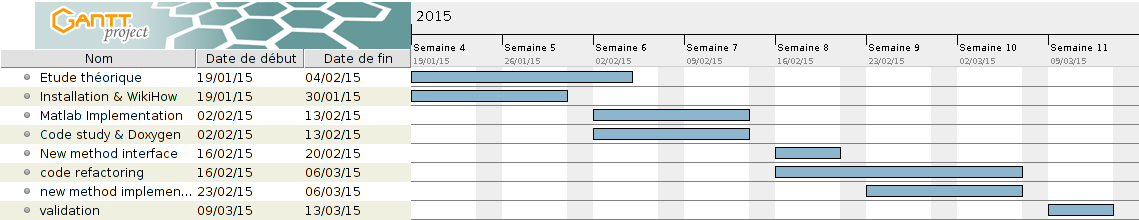
\includegraphics[width=1\textwidth]{Image/gantt.png}\centering
\caption{\textit{Initial gantt}}
\end{figure}
